%%%%%%%%%%%%%%%%%%%%%%%%%%%%%%%%%%%%%%%%%%%%%%%%%%%%%%%%%%%%%%%%%%%%%%%%%%%%%%%%%%
\begin{frame}[fragile]\frametitle{}
\begin{center}
{\Large Introduction}
\end{center}
\end{frame}


%%%%%%%%%%%%%%%%%%%%%%%%%%%%%%%%%%%%%%%%%%%%%%%%%%%%%%%%%%%
\begin{frame}[fragile]\frametitle{Calling the Call Center}
	\begin{itemize}
	\item Calling to an IVR (Integrated voice response)
	\item A prerecorded menu selection.
	\item ``Please press 1 for Account Details, Please press 2 for \ldots''
	\item till it comes to your option. 
	\item towards end, somewhere, given access to a person to talk to.
	\end{itemize}

Boring? Annoying?
\begin{center}
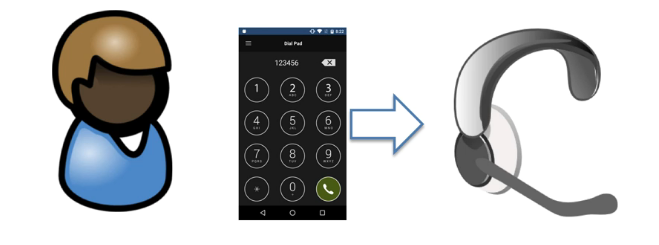
\includegraphics[width=0.6\linewidth,keepaspectratio]{nlp10}

\tiny{(Ref: Deep Learning and NLP A-Z - Kirill Eremenko)}
\end{center}
Instead, how about typing/saying your query directly and getting the answer right away?

\end{frame}

%%%%%%%%%%%%%%%%%%%%%%%%%%%%%%%%%%%%%%%%%%%%%%%%%%%%%%%%%%%
\begin{frame}[fragile]\frametitle{Solution}
Chatbots

	\begin{itemize}
	\item Which problem of IVR it is solving?
	\item Advantages?
	\item Disadvantages?
	\item Gaining popularity \ldots
	\item Many platforms
	\item Companies in Pune?
	\end{itemize}


\end{frame}

%%%%%%%%%%%%%%%%%%%%%%%%%%%%%%%%%%%%%%%%%%%%%%%%%%%%%%%%%%%
\begin{frame}[fragile]\frametitle{The Giants are at it \ldots}
\begin{center}
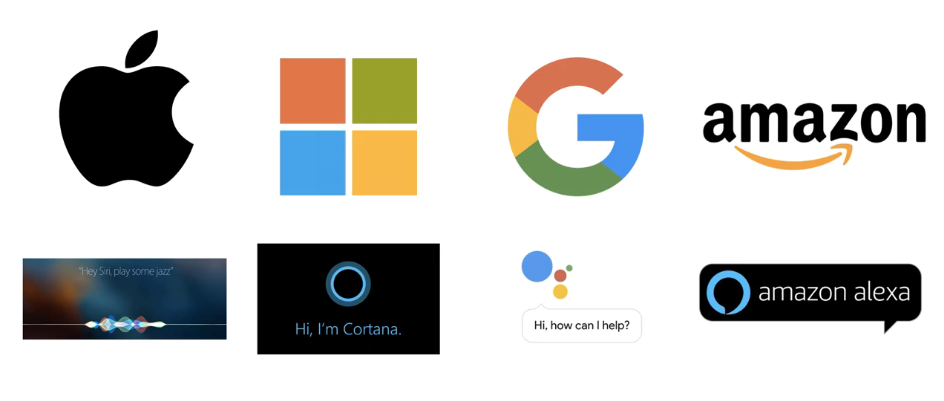
\includegraphics[width=0.8\linewidth,keepaspectratio]{nlp1}

\tiny{(Ref: Deep Learning and NLP A-Z - Kirill Eremenko)}
\end{center}

	\begin{itemize}
	\item Chatbots or QA systems, predominantly voice based, 
	\item Underlying processing is primarily Natural Language Processing (NLP).
	\item You can have your own chatbot, specific to you!! 
	\item NLP is the core skill needed.
	\end{itemize}
	
\end{frame}


%%%%%%%%%%%%%%%%%%%%%%%%%%%%%%%%%%%%%%%%%%%%%%%%%%%%%%%%%%%
\begin{frame}[fragile]\frametitle{Why so much popularity?}
Chatbots are:
	\begin{itemize}
	\item Autonomous and Always Available
	\item Drive Conversation
	\item Able to handle millions of requests, scalable.
	\end{itemize}
	
But to have a good Chatbot, at core, we would need expertize in NLP!!

\end{frame}


%%%%%%%%%%%%%%%%%%%%%%%%%%%%%%%%%%%%%%%%%%%%%%%%%%%%%%%%%%%
\begin{frame}[fragile]\frametitle{So, What is a Chatbot?}

\begin{itemize}
\item A chatbot is a computer program designed to simulate a conversation with human users, especially over the Internet.
\item A chatbot is meant to understand a human language, respond to it like a human and learn along the way to behave more human-ly.
\item Siri and Google assistant are classic examples of chatbots.
\end{itemize}

% {\tiny (Ref: Chatbots 101 - Architecture \& Terminologies -  Bhavani Ravi)}
\end{frame}

%%%%%%%%%%%%%%%%%%%%%%%%%%%%%%%%%%%%%%%%%%%%%%%%%%%%%%%%%%%
\begin{frame}[fragile]\frametitle{Why do we need a Chatbot?}

\begin{itemize}
\item Chat is the most natural way of interaction between human and application.
\item Bots are interactive.
\item Chatbots add a human touch to any application you build.
\item Bots are engaging. It is not as boring as filling up a long form.
\end{itemize}

% {\tiny (Ref: Chatbots 101 - Architecture \& Terminologies -  Bhavani Ravi)}
\end{frame}

%%%%%%%%%%%%%%%%%%%%%%%%%%%%%%%%%%%%%%%%%%%%%%%%%%%%%%%%%%%
\begin{frame}[fragile]\frametitle{Contextual Chatbot}

\begin{itemize}
\item Most chatbots today can handle simple questions and respond with pre-built responses based on rule-based conversation processing. 
\item For instance, if user says X, respond with Y; if user says Z, call a REST API, and so forth. 
\item High AI assistant is far more smater, it knows the context (previous chat history as well as sub domain)
\item Five levels of AI assistants: From notification assistants to autonomous organizations

\end{itemize}

% {\tiny (Ref: Chatbots 101 - Architecture \& Terminologies -  Bhavani Ravi)}
\end{frame}

% %%%%%%%%%%%%%%%%%%%%%%%%%%%%%%%%%%%%%%%%%%%%%%%%%%%%%%%%%%%
% \begin{frame}[fragile]\frametitle{AI Levels}
% Five levels of AI assistants: From notification assistants to autonomous organizations

% \begin{center}
% 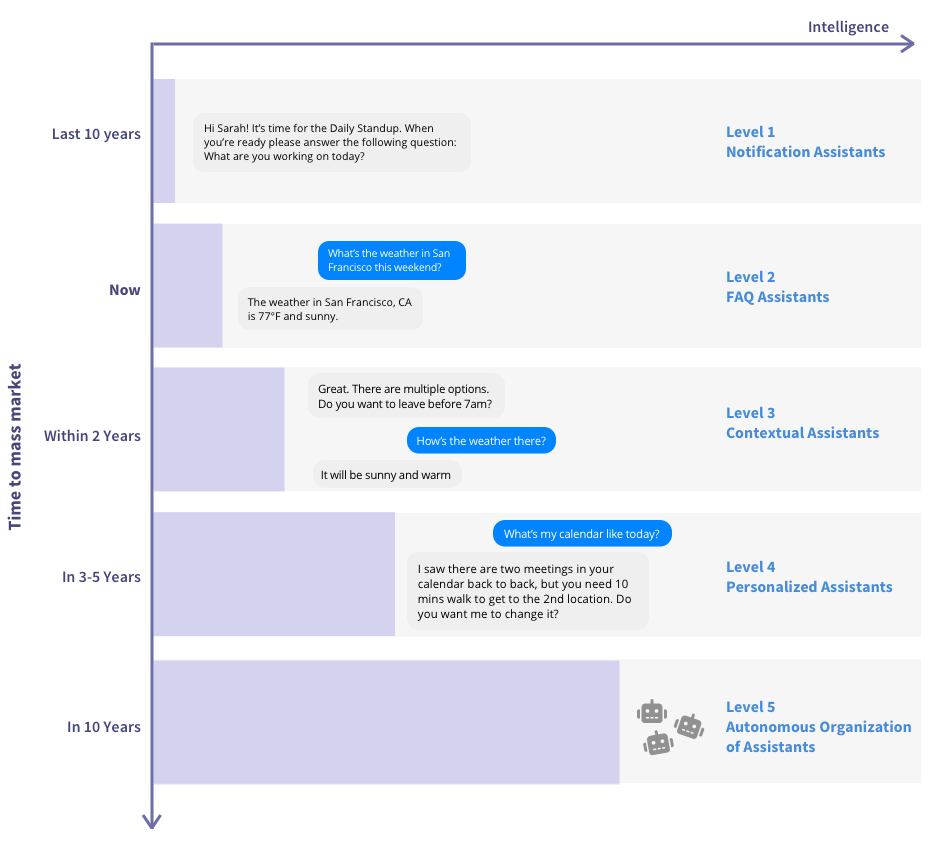
\includegraphics[width=0.6\linewidth]{chatbot1}
% \end{center}

% % {\tiny (Ref: The next generation of AI assistants in enterprise -  Alan Nichol)}
% \end{frame}

%%%%%%%%%%%%%%%%%%%%%%%%%%%%%%%%%%%%%%%%%%%%%%%%%%%%%%%%%%%
\begin{frame}[fragile]\frametitle{Level 1 : Notification Assistants}
\begin{itemize}
\item The chatbot is essentially a traditional notification assistant; it can answer a question with a pre-built response. 
\item It can send you notifications about certain events or reminders about things in which you’ve explicitly expressed interest. 
\item For instance, a level 1 travel bot can provide a link for you to book travel.
\end{itemize}

\begin{center}
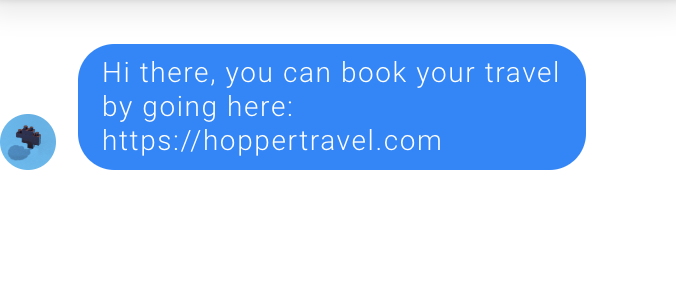
\includegraphics[width=0.6\linewidth,keepaspectratio]{chatbot13}
\end{center}

% {\tiny (Ref: The next generation of AI assistants in enterprise -  Alan Nichol)}
\end{frame}

%%%%%%%%%%%%%%%%%%%%%%%%%%%%%%%%%%%%%%%%%%%%%%%%%%%%%%%%%%%
\begin{frame}[fragile]\frametitle{Level 2 : FAQ Assistants}
\begin{itemize}
\item The chatbot can answer FAQs 
\item but is also capable of handling a simple follow up.
\end{itemize}

\begin{center}
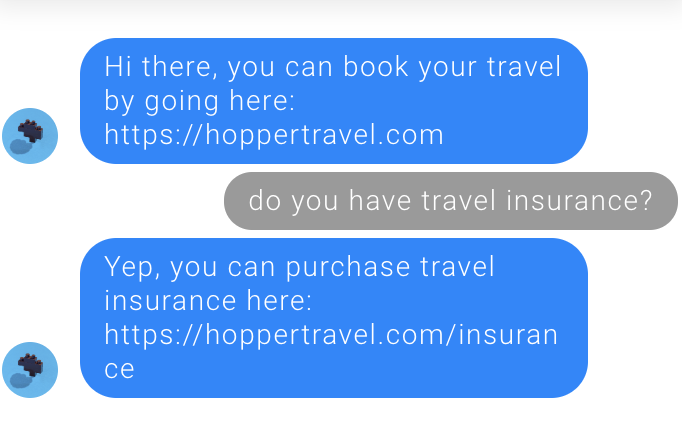
\includegraphics[width=0.6\linewidth,keepaspectratio]{chatbot14}
\end{center}

% {\tiny (Ref: The next generation of AI assistants in enterprise -  Alan Nichol)}
\end{frame}

%%%%%%%%%%%%%%%%%%%%%%%%%%%%%%%%%%%%%%%%%%%%%%%%%%%%%%%%%%%
\begin{frame}[fragile]\frametitle{Level 3 : Contextual Assistants}
\begin{itemize}
\item the contextual assistant can engage in a flexible back-and-forth with you and offer more than prebuilt answers because it knows how to respond to unexpected user utterances. 
\item The assistant also begins to understand context at this point. 
\item For instance, the travel bot will be able to walk you through a few popular destinations and make the necessary travel arrangements.
\end{itemize}

\begin{center}
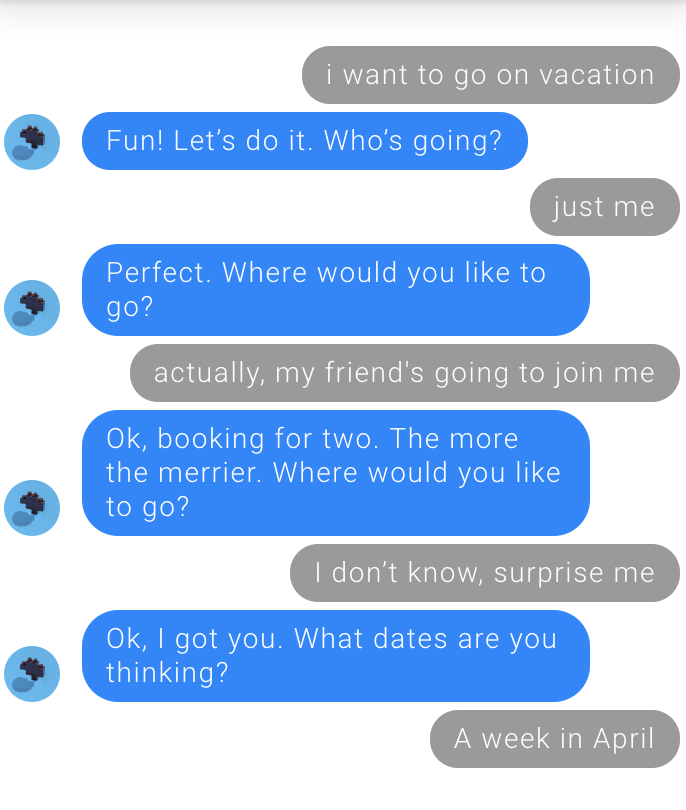
\includegraphics[width=0.6\linewidth,keepaspectratio]{chatbot15}
\end{center}


% {\tiny (Ref: The next generation of AI assistants in enterprise -  Alan Nichol)}
\end{frame}


%%%%%%%%%%%%%%%%%%%%%%%%%%%%%%%%%%%%%%%%%%%%%%%%%%%%%%%%%%%
\begin{frame}[fragile]\frametitle{Level 4 : Personalized Assistants}
\begin{itemize}
\item the contextual assistant can engage in a flexible back-and-forth with you and offer more than prebuilt answers because it knows how to respond to unexpected user utterances. 
\item The assistant also begins to understand context at this point. 
\item For instance, the travel bot will be able to walk you through a few popular destinations and make the necessary travel arrangements.
\end{itemize}

\begin{center}
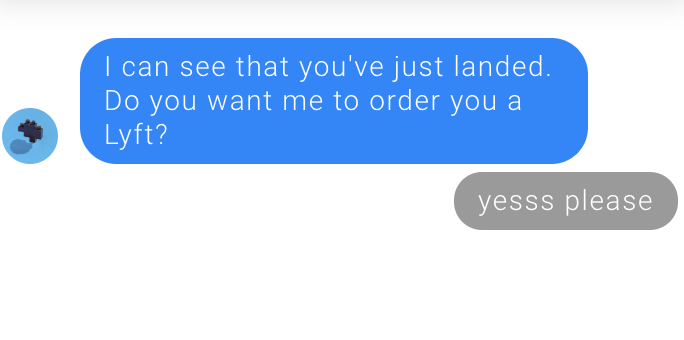
\includegraphics[width=0.6\linewidth,keepaspectratio]{chatbot16}
\end{center}

% {\tiny (Ref: The next generation of AI assistants in enterprise -  Alan Nichol)}
\end{frame}

%%%%%%%%%%%%%%%%%%%%%%%%%%%%%%%%%%%%%%%%%%%%%%%%%%%%%%%%%%%
\begin{frame}[fragile]\frametitle{Level 5 and beyond: Autonomous Organization of Assistants}
\begin{itemize}
\item contextual assistants are able to monitor and manage a host of other assistants in order to run certain aspects of enterprise operations. 
\item They’d be able to run promotions on certain travel experiences, target certain customer segments more effectively based on historical trends, increase conversion rates and adoption, and so forth.
\end{itemize}


% {\tiny (Ref: The next generation of AI assistants in enterprise -  Alan Nichol)}
\end{frame}


%%%%%%%%%%%%%%%%%%%%%%%%%%%%%%%%%%%%%%%%%%%%%%%%%%%%%%%%%%%
\begin{frame}[fragile]\frametitle{Conversational Chatbot}

\begin{itemize}
\item Understands the context of the conversation
\item Can handle any user goal gracefully
\item Means that the bot may not be able to answer all questions but it can handle the conversation well.
\end{itemize}

Simple conversation:
\begin{center}
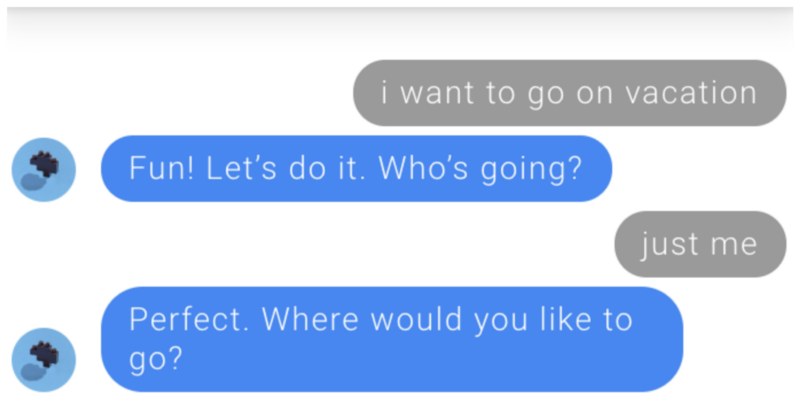
\includegraphics[width=0.6\linewidth,keepaspectratio]{chatbot17}
\end{center}


\end{frame}

% %%%%%%%%%%%%%%%%%%%%%%%%%%%%%%%%%%%%%%%%%%%%%%%%%%%%%%%%%%%
% \begin{frame}[fragile]\frametitle{How are chatbots different from Apps?}

% \begin{itemize}
% \item Chatbots are the most natural way of interaction, it just feels like asking your friend for help but can still do all the activities that a has to do.
% \item Chatbot is like adding a conversational interface to apps.
% \end{itemize}

% {\tiny (Ref: Chatbots 101 - Architecture \& Terminologies -  Bhavani Ravi)}
% \end{frame}

